% !TeX spellcheck = en_US
\documentclass[RAIstudentthesis%      style
              ,optCharter%            font
              ,optBlackHeadings%      black sections to reduce number of colored pages
              ,optBlackRefs%          black references to reduce number of colored pages
              %,optCMYK%              color model
              ,optBiber% 	          bibliography tool
              ,optBibstyleAlphabetic% bibliography style
              ,optCenterEquations%    alignment of equations
              ,optEnglish% 		      language
              %,optTikzExternalize%   compiles faster for large tikz images
              %,optExzellenz%
              ]{RAIlatex}
%
% Load other LaTeX packages
\usepackage{booktabs}%
\usepackage[acronym, toc, shortcuts]{glossaries}
\usepackage{array}
%
% Set paths
\graphicspath{{figures/}}%
\addbibresource{safety_offloading.bib}%
%
% Define additional commands
\newcommand{\code}[1]{\texttt{#1}}%
\newcommand{\degree}[0]{^\circ}%
%
% make glossaries
\makeglossaries
%


\begin{document}
% Titlepage
% ---------
\frontmatter%
% Info: separate multiple supervisors by \newline
%\RAIstudentthesisTitlePageCustomDiplomarbeit{German Title}{English Title}{\RAIlangFieldOfStudyRoboticsCognitionIntelligence}{Martin Mustermann}{}{\RAInamesProfKnoll}{Musterbetreuer, M.Sc.}{\RAIutilsDate{1}{1}{2020}}%
%\RAIstudentthesisTitlePageCustomBachelorsThesis{German Title}{English Title}{\RAIlangFieldOfStudyRoboticsCognitionIntelligence}{Martin Mustermann}{}{\RAInamesProfKnoll}{Musterbetreuer, M.Sc.}{\RAIutilsDate{1}{1}{2020}}%
%\RAIstudentthesisTitlePageCustomSemesterThesis{German Title}{English Title}{\RAIlangFieldOfStudyRoboticsCognitionIntelligence}{Martin Mustermann}{}{\RAInamesProfKnoll}{Musterbetreuer, M.Sc.}{\RAIutilsDate{1}{1}{2020}}%
%\RAIstudentthesisTitlePageCustomIDP{German Title}{English Title}{\RAIlangFieldOfStudyRoboticsCognitionIntelligence}{Martin Mustermann}{}{\RAInamesProfKnoll}{Musterbetreuer, M.Sc.}{\RAIutilsDate{1}{1}{2020}}%
\RAIstudentthesisTitlePageCustomMastersThesis{Analyse von Edge Computing Offloading Strategien für autonome mobile Roboter}{Analysis of Edge Computing Offloading Strategies for Autonomous Mobile Robots}{\RAIlangFieldOfStudyRoboticsCognitionIntelligence}{Xiyan Su}{}{\RAInamesProfKnoll}{Robin Dietrich, M.Sc.}{\RAIutilsDate{15}{05}{2023}}%
%
% Abstract
% --------
% In total max. 1 Page!
\RAIstudentthesisAbstract{%
%
% Abstract English:
To achieve autonomy, \acp{amr} need to run different computation and memory intensive algorithms, such as perception, \ac{slam}, path planning, and learning. However, an \ac{amr}'s on-board computational and energy resources are limited by space restrictions and battery lifetime. With the emergence of edge computing, \acp{amr} have the opportunity to offload costly computation tasks to the edge, while only a small portion of the computation remains on the on-board system. However, depending on the application scenarios, offloading certain tasks from the \ac{amr} to the edge at all times may not be possible, beneficial or even feasible due to the network's latency, dynamic network changes, and resource availability. On the other hand, offloading computational workloads to the edge could impact the robot's safety, availability as well as on-board resources. The exact influence on the robotic system will depend on the chosen offloading strategy. Therefore, this thesis uses object detection as an offloading task and investigates the performance and the latency, as well as the CPU usage and power consumption of the robot's on-board system under diffferent offloading strategies. 
% Furthermore, this thesis implements a decision-making offloading strategy based on the network conditions and robot's on-board system states to minimize the latency, but is also subjected to restrictions of the power consumption and CPU usage.
}{%
%
% Zusammenfassung Deutsch:
Die autonomen mobilen Roboter müssen verschiedene rechnen- und speicherintensive Algorithmen ausführen. 
}%
%
%
%

%
% List of figures and tables
% --------------------------
\listoffigures
\listoftables

%
% Glossaries
% ----------
\newglossaryentry{docker}{
    name=Docker,
    description={Docker}
}

\newglossaryentry{gazebo}{
    name=Gazebo,
    description={Gazebo}
}

\newglossaryentry{linux}{
    name=Linux,
    description={Linux}
}

\newglossaryentry{wifi}{
    name=Wi-Fi,
    description={Wi-Fi}
}

\newacronym{netem}{NetEm}{Network Emulator}

\newacronym{amr}{AMR}{Autonomous Mobile Robot}

\newacronym{ai}{AI}{Artificial Intelligence}

\newacronym{mec}{MEC}{Multi-Access Edge Computing}

\newacronym{slam}{SLAM}{Simultaneous Localization and Mapping}  

\newacronym{mcc}{MCC}{Multi-Access Cloud Computing}

\newacronym{hrc}{HRC}{Human-Robot Collaboration}

\newacronym{ros}{ROS}{Robot Operating System}

\newacronym{nuc}{NUC}{Intel Next Unit of Computing}

\printglossary
%
% Content
% -------
\RAIstudentthesisPrintTableOfContents%
\mainmatter%
\chapter{Questions Need to Be Answered}

\begin{itemize}
    \item why choose object detection as a offloading task? 
    \item why is mean average precision is a metric
    \item why choose NUC as the robotic platform? How can NUC represent a normal robot computing system?
    \item How is a ROS bag replay represents the camera on the robot?
\end{itemize}
% !TeX spellcheck = en_US
\chapter{Introduction}\label{ch:introduction}

This chapter first gives the context of the thesis and introduces the research problem the thesis addresses. Furthermore, this chapter discusses the research questions the thesis is trying to answer and what approaches the thesis adopts to investigate these questions.

\section{Background}\label{sec:introduction:background}

\glspl{amr} have gained enormous significance in automated factories. Recent developments in robotics and \gls{ai} have enabled the \gls{amr} to operate with autonomy. This requires the \glspl{amr} to run computation- and memory-intensive algorithms related to image processing, path planning, \gls{slam}, and learning \cite{Saeik2021}. However, \citeauthor*{Baxi2022} point out this poses a challenge for the robot's onboard system, which has limited computational capabilities due to size and cost limitation as well as battery life. Furthermore, these algorithms are time-sensitive and can cause operational failure for the \glspl{amr} if the latency restrictions cannot be satisfied. It becomes essential for large automated factories using \glspl{amr} to address this problem. 

% Maybe mention Human-Robot Collaboration?

\begin{figure}[htb]
    \centering

    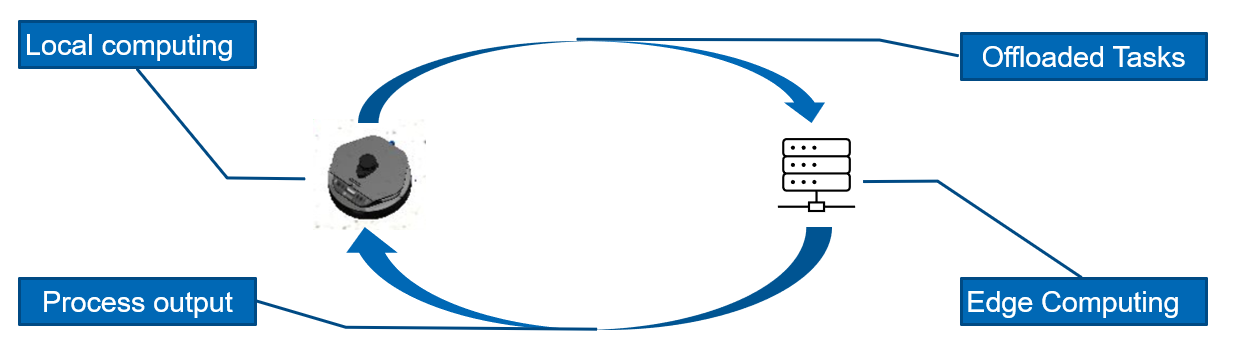
\includegraphics[width=120mm]{figures/setup/amr_offloading.png}
    \caption{Offloading pipeline between \gls{amr} and edge computer}

    \label{fig:amr_offloading}
\end{figure}

\gls{mec} as an evolution of \gls*{mcc} brings application hosting from data centers down to the edge of the network, where the data were initially collected, to achieve low latency and bandwidth efficiency \cite{Lin2019}. For latency-sensitive tasks on \glspl{amr}, such as perception and navigation, \gls{mec} offers an opportunity to enable the \glspl{amr} with limited resources by offloading costly computation tasks to the edge, while only a small portion of the computation remains on the \gls{amr}'s on-board system. A full offloading pipeline for \glspl{amr} is illustrated in figure~\cref{fig:amr_offloading}.


However, depending on the application scenarios, offloading certain tasks from the \glspl{amr} to the edge at all times may not be possible, beneficial or even feasible due to the network's latency, dynamic network changes, and resource availability. \citeauthor*{Baxi2022} point out that a simple perception task using an RGB-D camera can cause over 100 ms sensing-to-actuation round-trip latency and over 50 MBytes per second network bandwidth usage. On the other hand, offloading computational workloads to the edge could also impact the \gls{amr}'s safety, availability as well as on-board resources. The exact influence on the robotic system will depend on the chosen offloading strategy. Therefore, it is necessary to investigate the effects of certain offloading strategies on the \gls{amr}'s safety, availability, and task performance.

\section{Research Questions}\label{sec:introduction:research_questions}

This thesis first implements an offloading framework for robot perception and analyzes the effects of different offloading strategies, using \gls{ros} \cite{Macenski2022}. More specifically, this thesis considers a 2D object detection task using YOLOv5 network, proposed by \citeauthor*{Jocher2020}. YOLOv5n, a smaller variant of the perception network, will be deployed on the \gls{amr}'s on-board system, while the edge counterpart uses a more accurate but also more complex variant, e.g., YOLOv5l. The environment is an industrial warehouse containing human objects as obstacles. The \glspl{amr} are equipped with camera sensors and use the native \gls{ros} navigation stack, proposed by \citeauthor*{Macenski2020} to navigate from a user-defined route. 

This thesis first investigates offloading strategies with different offloading ratios. The \gls{amr} offloads a portion of the incoming frames from the camera to the edge computer with different offloading ratios incrementing from 0 percent to 100 percent with a stepping of 10 percent, i.e., the \gls{amr} offloads 10, 20, ..., 80, 90 percent of the incoming frames to the edge computer. At 0 percent, the \gls{amr} does not offload at all to the edge computer and only relies on its onboard resources. At 100 percent, the \gls{amr} does not perform any local computation and only relies on the computation output of the edge computer. This step aims to investigate the influence of different offloading strategies on the performance of the perception task and the resource usage of the \gls{amr} and the edge computer as well as the network. Then, this thesis carries on to implement a decision-making offloading strategy depending on run-time parameters, such as latency and \gls{amr}'s CPU usage and power consumption. This strategy is a simplified variant of the algorithm proposed by \citeauthor*{Ning2019} with a goal of minimizing latency and additional constraints subjected to power consumption and network bandwidth. 

This thesis evaluates the aforementioned offloading strategies regarding different metrics such as the CPU usage and power consumption of the \gls{amr}, the network bandwidth in use, and the mean average precision of the 2D object detection algorithm for human obstacles. The offloading strategies are first evaluated in simulation and later on in real robotic systems. With the results from these experiments, this thesis is trying to answer the following research questions: What effects do the aforementioned offloading strategies have on the specified metrics? Furthermore, this thesis is trying to answer the question: If and how the effects of different offloading strategies vary under different circumstances and if they have any (application-specific) constraints.Finally, this thesis is trying to gain insights if more complex strategies to achieve better results on the metrics. 

\section{Methodology}\label{sec:introduction:methodology}

This thesis first implements a reliable framework for \glspl{amr} using object detecting task as an example and using \gls{ros} as middleware. Then, the thesis implements a simulation scenario in \gls{gazebo}. The implemented scenario simulates a factory warehouse including obstacles such as shelves, boxes, and human. Finally, this thesis improves the object detection pipeline in order to achieve the real-time inference on both the \gls{amr}'s onboard system and the edge computer. The thesis intends to investigate the influence of different offloading strategies. Therefore, an inference pipeline with real-time inference capabilities reduces the performance requirements for both the \gls{amr}'s onboard system as well as the edge computer.

% glossary for "docker" and "netem"
With the aforementioned ground works in place, this thesis first conduct the experiment in simulation using \gls{ros} and \gls{netem}. Then, this thesis continues to conduct the experiment on real robotic system with \gls{wifi} and Ethernet connection to the edge computer. In order to achieve consistent and comparable results, the simulation experiment and the real-robot experiment use the same simulation scenario recording. Therefore, the inputs of the real-robot experiment are not collected from real world using camera sensors. However, this thesis shows that the performance overhead of the replay of the simulation data is comparable with the camera sensor module on the \gls{amr}. The comparison will be elaborated in~\cref{ch:real_robot_experiment}. 

The experiment results from the simulation and the real-robot experiments are evaluated after the execution of the experiment using the data collected during the experiment in order to reduce the influence of the data collection on the performance of the \gls{amr}'s onboard system and the edge computer.

\section{Structure of the Thesis}

In ~\cref{ch:background}, this thesis gives an introduction to the related works that are needed to understand the content of the thesis. In ~\cref{ch:general_setup}, this thesis describes in details the implementation of the offloading framework this thesis uses to investigate the research questions. It also describes the implementation of the offloading strategies. Furthermore, this thesis presents the evaluation methods for different evaluation metrics. In ~\cref{ch:simulation} and ~\cref{ch:real_robot_experiment}, this thesis describes how the experiments are conducted in simulation as well as on real robotic system. Moreover, this thesis analyzes the results and discusses the experiments. Finally, in ~\cref{ch:conclusion_and_future_works}, this thesis gives the conclusion to the research questions and discusses the limitation of the works 

% !TeX spellcheck = en_US
\chapter{Background}

\section{Autonomous Mobile Robot}
\subsection{Development}
\subsection{Perception}
\subsection{SLAM}
\subsection{Path Planning}
\subsection{ROS}
\subsection{Turtlebot}

\section{Multi-access Edge Computing}
% could mention TSN (time sensitive network)
\subsection{Cloud Computing}
\subsection{Fog Computing}
\subsection{Edge Computing and IoT}

\section{Related Works}
\subsection{Purposes}
\subsection{Metrics}
\subsection{Decision-making-based Strategies}
\subsection{Learning-based Strategies}

\chapter{Algorithms}\label{ch:algorithms}
\chapter{General Setup}\label{ch:general_setup}

This chapter describes the implementation of the offloading framework in use. However, since this thesis conducts experiments both in simulation and on real robot, there are technical differences between the actual software setups. To avoid redundancies, this chapter introduces the general offloading setup in \cref{sec:general_setup:implementation} that is mutually adopted by the two setups. Furthermore, \cref{sec:general_setup:offloading_strategies} also describes the algorithms that are used to realize different offloading strategies. 
Finally, in \cref{sec:general_setup:evaluation}, this chapter discusses the evaluation paradigm in use for different evaluation metrics.

\section{Implementation}\label{sec:general_setup:implementation}

This thesis implements an offloading pipeline for a robotic object detection task. This includes an offloading module making decision whether to offloading the image from the camera sensor to the edge computer or to compute the image locally using onboard resources. An inference pipeline for object detection task is implemented using pre-trained models from YOLOv5 \cite{Jocher2022} deployed using PyTorch library \cite{Paszke2019}. Furthermore, in order to test the offloading framework in repeatable and comparable experiments, a simulation scenario is implemented in \gls{gazebo} \cite{Koenig2004} and a recording of the scenario run is created with \gls{ros}. Finally, since the output of the object detection task is not used in any downstream applications. This thesis considers and implements various evaluation paradigms to retrieve meaningful results from the data collected during the experiments. To delimit, this thesis only investigates the scenario where one \gls{amr} offloads to one edge computer. Investigations for multi-robot multi-edge scenarios are beyond the scope of this thesis. 

\subsection{Offloading Module}

\begin{figure}[htp]
    \centering
    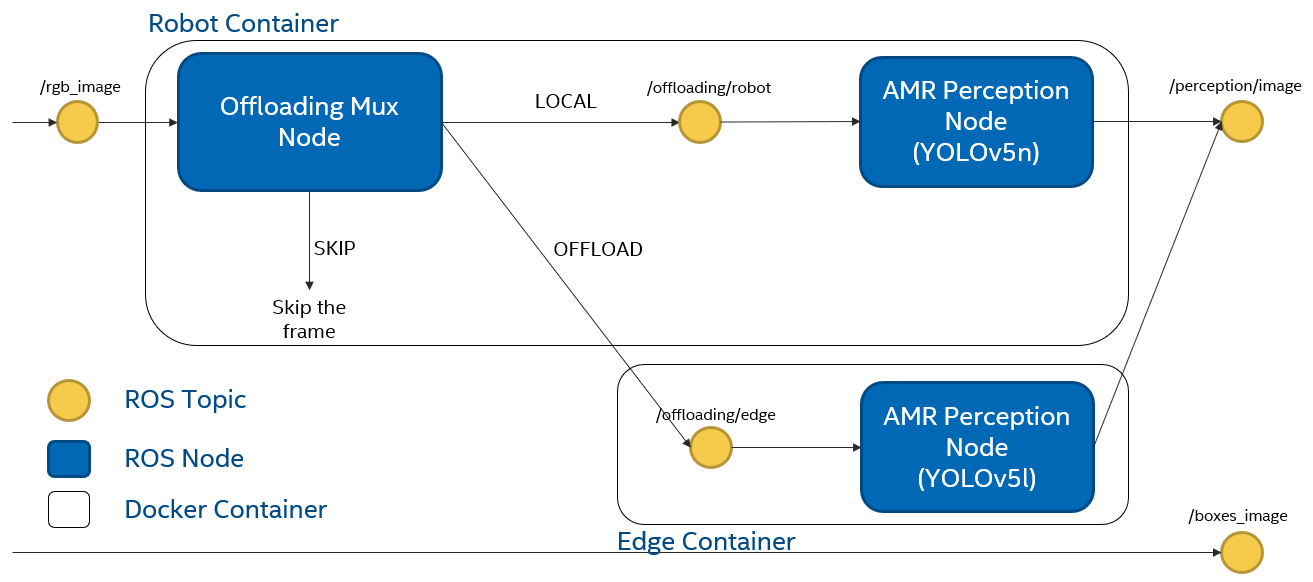
\includegraphics[width=120mm]{figures/setup/general_setup.png}
    \caption{General Setup (TODO: adapt this image)}
    \label{fig:general_setup}
\end{figure}

% TODO: this may need some adaptions to the dynamic offloading module
An offloading pipeline should have the abilities to make decision, coordinate the resources and communicate over the network. A generic offloading pipeline is illustrated in~\cref{fig:general_setup}. Each blue block represents a \gls{ros} node and each yellow circle represents a \gls{ros} topic. The arrows indicate the directions of the data flow. The dotted lines are the virtualization of the robotic system and the edge computer. The images can come from either a camera sensor or the replay of the simulation scenario. Once the \gls{amr} receives the image, the offloading module will have to decide whether to offload the image to the edge computer or pass it to the local perception node, which uses a simpler and lighter model for image inference. The offloading module makes offloading decisions by publishing the received image to pre-defined \gls{ros} topics. Once the perception nodes receive the image, they will start to do inference on the given image. Then, the processed results are published to another pre-defined \gls{ros} topic and recorded by the \gls{ros} bag. Meanwhile, the ground truth of the simulation for the object detection task is also published to a \gls{ros} topic and recorded by the \gls{ros} bag. 

In order to evaluate different offloading strategies, the offloading module possesses the ability to switch between them. Therefore, the offloading strategies act as plugins for the offloading module. Furthermore, the offloading module is responsible for loading the static hyper-parameters for the offloading strategies on start-up and also for keeping track of the run-time states of the system to allow dynamic offloading strategies. In an offloading pipeline, the system states come from various \gls{ros} nodes observing different functionalities of the system. This information is published to different \gls{ros} topics and subscribed by the offloading module. To reduce the influence of the fluctuation in the observed system states, the offloading module applies a \gls{sma} algorithm to smooth the data. 

Since the offloading pipeline is built upon the \gls{ros}, the behaviour of \gls{ros} and its underlying technical realization is crucial to the behaviour of the offloading pipeline, such as \gls{dds} and \gls{qos} settings. The exact influence of these settings on the behaviour of the offloading pipeline and the performance of the offloading will be discusses in \cref{ch:simulation} and \cref{ch:real_robot_experiment}. 

\subsection{Perception Module}

% discuss the choice of synchronous inference and asynchronous inference. Also defend not retraining the model.

% TODO: find the quote on the edge computers
In general, an offloading task can be any computationally intensive algorithms the \gls{amr} is required to run, such as perception, navigation, \gls{slam}, path planning, etc. This thesis chooses an object detection task as an example, because an object detection task can have significant performance difference between the \gls{amr}'s onboard system and the edge computer, which corresponds to the usage scenario of the edge offloading. An \gls{amr} is usually equipped with a simple onboard system with only access to \gls{cpu}, while an edge computers are usually cloudlets and data centers on premise with access to \gls{gpu}. As mentioned in \cref{ch:background}, the \glspl{amr} use primarily \glspl{dnn} to detect objects. With frameworks like PyTorch that can make use of the \gls{gpu}, the performance difference between \gls{amr}'s onboard system and the edge computer is immense. Therefore, this thesis chooses the object detection as an example for offloading tasks. 

% TODO: fill in the real value
\begin{table}[htb]%
    \centering%
    \begin{tabular}{lccccc}
        \toprule
        Model &                     YOLOv5n &   YOLOv5s &   YOLOv5m &   YOLOv5l &   YOLOv5x \\
        \midrule
        Robot inference time &      0.0 ms &    0.0 ms &    0.0 ms &    0.0 ms &    0.0 ms  \\
        Edge inference time &       0.0 ms &    0.0 ms &    0.0 ms &    0.0 ms &    0.0 ms  \\
        Model size &                0 MB &      0 MB &      0 MB &      0 MB &      0 MB    \\
        \gls{map} &                 45.7\% &  56.8\% &    64.1\% &    67.3\% &    68.9\%  \\
        \bottomrule
    \end{tabular}
    \caption{Inference times of different YOLOv5 models on \gls{amr}'s onboard system and edge computer}
    \label{tab:inference_time}%
\end{table}

% TODO: ask if it's okay to list the hardware specification
% TODO: better phrasing
In order to adapt to the performance difference between the \gls{amr}'s onboard system and the edge computer, the perception module should have two models available for object detection: a lightweight model that runs on the onboard system and a more complex model that runs on the edge computer. \gls{yolov5} provides a series of models with different complexities. To find appropriate models for the onboard system and the edge computer, this thesis investigates the inference times of different models on different machines, which can be taken from \cref{tab:inference_time}. To simulate the computation capability discrepancy between the two systems, this experiment uses a \gls{nuc} equipped with an Intel(R) Core(TM) i3-8109U \gls{cpu} and without access to \gls{gpu}. On the other hand, the edge computer is equipped with an Intel(R) Core(TM) i9-7900X \gls{cpu} and equipped with Nvidia GeForce GTX 1060 6GB \gls{gpu}. The models are deployed with \gls{pytorch} and output an array of bounding box detections. The inference time is measured between the time when the \gls{yolov5} receives the image and the time when the perception node outputs an array of bounding box detections. This includes the time for image pre-processing and the time of results post-processing. Furthermore, the image input for the offloading module has a frame rate has an average of 30 frames per second. To achieve real time, it is necessary that the inference time does not exceed 100 ms (\textbf{\textit{maybe phrase it better here}}). Longer inference time also cause the actual precision of the object detection to deteriorate, which will be discusses in \cref{sec:general_setup:evaluation}. The model sizes and the \gls{map} data are taken from the the documentation from \citeauthor*{Jocher2022} \cite{Jocher2022}. The \gls{map} data are evaluated on \gls{coco} val2017 \cite{Lin2014}. As a compromise between the inference time and the performance, this thesis chooses to deploy \gls{yolov5}n on the \gls{amr}'s onboard system and \gls{yolov5}l on the edge computer. 

To delimit, the object detection models in use are pre-trained and not re-trained with custom data from the simulation. This thesis intends to investigate different offloading strategies and generating custom data-sets and re-training the models are laborious tasks. Therefore, a re-training of the models is beyond the scope the this thesis. \citeauthor*{Jocher2022} \cite{Jocher2022} state that the all pre-trained models are trained on \gls{coco} data-sets for 300 epochs with default settings. Moreover, this thesis only considers human obstacles, which is a detection class in \gls{coco} data-sets. Therefore, the pre-trained models can provide comparability between different offloading strategies on different machines. Furthermore, re-training of the models is dependent on the quality and the size of the custom data-sets. An improper re-training can introduce additional errors or over-fitting of the models and thus undermine the comparability. 

\subsection{State Monitor}

To evaluate different offloading strategies, this thesis need to get access to the system states, such as the \gls{cpu} usage, energy consumption, and network bandwidth. Various modules are implemented to measure them. 
The measurements from these modules are recorded for evaluation and also used for dynamic strategies that making decision based on run-time states of the system. However, in simulation experiments, the virtualization of the \gls{amr}'s onboard system and the edge computer is realized by the \gls{docker} containers. In contrast, different physical computers are used in the real-robot experiments. This difference in the system virtualization affects how the system states are measured. 

For simulation experiments, \gls{docker} provides the containerized system virtualization and virtual network interfaces. \citeauthor*{Ruggeri2022} \cite{Ruggeri2022} proposes that the network bandwidth in use can be measured with the network throughput. The network throughput and \gls{cpu} usage can be measured with the the statistics of the \gls{docker} containers, which is a functionality provided by \gls{docker}. Alternatively, the system states of containers can be monitored using \gls{cadvisor}. For real-robot experiments, the \gls{cpu} usage and the network throughput are measured separately on different machines using \gls{psutil} tools. In the case of Intel \glspl{cpu}, the power consumption can be measured with \gls{rapl} provided by \gls{linux} kernel Power Capping Framework. \citeauthor*{Xie2021} \cite{Xie2021} propose that the execution latency of the offloading task consists of two components: the network delay and the inference time. The network delay measures the time needed for transferring the data from the offloading module to the perception module, while the inference time measures the time the perception module need to process the inference, including the time for image pre-processing and result post-processing. The execution latency is measured with timers residing in the offloading module and and the perception module. The timers record the time stamps to critical time points in the transfer and inference process and calculate the time difference. Then, the data are published to a \gls{ros} topic and can be access by other subscribers. 

% TODO: not sure if this paragraph is necessary
Since it is assumed that the edge computer has abundant resources, the system states of the edge computer are not measured and are not taken into consideration during the decision-making and the evaluation process. Furthermore, even though this thesis only investigates the single-robot single-edge scenario, the available resources from the edge computers can be affected by numerous factors in real-world applications, such as the number of edge computers, the number of \glspl{amr}, and other processes running the edge computers. In addition, with more powerful hardware and easy access to power supply, the edge computer consumes more energy and computation resources for the same task than the \gls{amr}'s onboard system. Therefore, it is pointless to compare the consumption of the resources between two systems with na\"{i}vet\'{e}. In contrast, the network connection between the \gls{amr} and the edge computer is fragile and prone to disturbance. Therefore, this thesis only considers the system states of the \gls{amr}'s onboard system and the network condition between the \gls{amr} and the edge computer. 

\subsection{Offloading Strategies}\label{sec:general_setup:offloading_strategies}

Offloading strategies decides how the \gls{amr} offloads the computation task to the edge computer and have influence on various metrics of the system. Therefore, they are the core of the this thesis. As baselines, this thesis first investigates the scenarios where the \gls{amr} only computes the object detection task locally on its onboard system or only offloads the task to the edge computer. Then, the thesis continues to investigate the scenarios where the \gls{amr} offloads a portion of the frames with a fixed ratio. The offloading strategies with a fixed offloading ratio can be realized with \cref{alg:ratio_strategy}. The offloading ratio should be a value ranging from 0 to 1. Any offloading ratios greater 1 will cause the offloading module only to offload to the edge computer. Accordingly, any negative offloading ratios will cause the offloading module only to compute locally. With results from the experiments on baseline offloading strategies, this thesis intends to find the limits of the system and analyze its behaviour. 


% This sections describes how RobotOnlyStrategy, EdgeOnlyStrategy, RatioStrategy are implemented. Include a psuedo algorithms here for RatioStrategy
\begin{algorithm}[htp]
\caption{Algorithm to offload with a fixed ratio}\label{alg:ratio_strategy}
\begin{algorithmic}[1]
    \Function{RatioStrategy}{$r$} \Comment{where r is the offloading ratio}
        \State $c_1 \gets \, $GetImageCounter()\Comment{Get the counter for the total images received}
        \State $c_2 \gets \, $GetOffloadCounter()\Comment{Get the counter for the images offloaded}
        \State SetImageCounter($c_1 + 1$) \Comment{Add one first to image counter to avoid zero division}
        \If{$c_2 / c_1 \ge r$}
            \State return false \Comment{Compute locally}
        \Else
            \State SetOffloadCounter($c_2 + 1$)
            \State return true \Comment{Offload to edge computer}
        \EndIf
    \EndFunction
\end{algorithmic}
\end{algorithm}

Dynamic offloading strategies use the run-time system states to decide whether to offloading. They can adapt to the dynamic changes of the system and the network. With the results from the baseline offloading strategies, this thesis continues to investigate one dynamic strategy. More specifically, a simple version of the offloading strategy proposed by \citeauthor*{Ning2019} \cite{Ning2019} with the goal of minimizing the execution latency. Moreover, this dynamic offloading strategy is subjected to constraints of other system states. In this thesis, we consider two run-time system states as constraints: \gls{amr}'s \gls{cpu} usage and the network throughput. The problem can be formulated as a constraint optimization problem as follow:

\begin{equation}
    \min_{(\alpha, \beta)} \: t_{latency} = t_{inference} + t_{network}
\end{equation}

with

\begin{equation*}
    t_{inference} = \alpha t_{inference}^{L} + \beta t_{inference}^{E}
\end{equation*}
\begin{equation*}
    t_{network} = \alpha t_{network}^{L} + \beta t_{network}^{E}
\end{equation*}

s.t.

\begin{equation*}
    \alpha + \beta = 1
\end{equation*}

\begin{align*}
    & \alpha = \begin{cases}
        1, & \text{if the task is processed locally} \\
        0, & \text{else.}
    \end{cases} \\
    & \beta = \begin{cases}
        1, & \text{if the task is processed by the edge computer} \\
        0, & \text{else.}
    \end{cases}
\end{align*}

where the $t_{latency}$ represents the overall execution latency of the object detection task and $t_{inference}$ and $t_{network}$ represent the inference time and the network delay correspondingly. 

In addition to the execution latency, the offloading decision is also subjected to the \gls{amr}'s \gls{cpu} usage and the network throughput. If the \gls{cpu} usage exceeds certain value, the \gls{amr} only offloads to the edge. Similarily, the \gls{amr} only computes the task locally if the network throughput exceeds the threshold. These constraints ensure that the \gls{amr} and the network are capable of finish the task at all. The decision-making strategy can be implemented as 

\begin{algorithm}[htp]
\caption{Algorithm to offload with dynamic parameters}\label{alg:decision_making_strategy}
\begin{algorithmic}[1]
    \Function{DecisionMakingStrategy}{$r, params$}\Comment{offloading ratio: $r$, run-time parameters: $params$}
        \Comment{add an algorithm here.}
    \EndFunction
\end{algorithmic}
\end{algorithm}



\section{Simulation}\label{sec:general_setup:simulation}

To run experiments both in simulation and on real robots, this thesis implements a simulation scenario of a factory warehouse with one \gls{amr} and obstacles. The simulation is recorded and replayed for each experiment run to reduce the computation overhead of the simulation and to make the experiment repeatable. Furthermore, in order to compare the results from simulation and real robot, the simulation recording is used as input for both experiments under the same replay settings. 

\subsection{Simulation scenario}

% include a bird-view shot for the simulation with warehouse, robot, and human obstacles in the view.
The scenario simulates a modern-day factory warehouse, illustrated in (refer to the figure here). The simulated scenario is implemented in \gls{gazebo} with the help of a software package called "scenario execution", which the author implemented during his work at Intel Labs. The scenario consists of a factory warehouse environment and static obstacles, such as humans, boxes, shelves, and pallets, which are common obstacles in a factory warehouse. Since the object detection models are pretrained with \gls{coco} data-sets, which do not contain many of the static obstacles. The evaluation for the \gls{map} is of the object detection task is restricted only to detect the human obstacles. To clarify, the object detection models still detect all of the classes that are defined in the \gls{coco} data-sets. However, only the human class is taken into considering when calculating the \gls{map} metric during the evaluation. Since the performance difference among different \gls{yolov5} models are negligible when the scene is too simple, this thesis includes ten human obstacles in the simulation scenario to increase the complexity of the object detection task. Moreover, some human obstacles are occluded by other obstacles in the scenario. Detecting occluded objects has been proven to be a challenging task in object detection. 

% \begin{figure}
%     \centering
%     \includegraphics[width=120mm]{}
%     \caption{Bird view of the simulation scenario}
%     \label{fig:bird_view_scenario}
% \end{figure}

The \gls{amr} is implemented as a dynamic obstacle in the scenario and it moves along a pre-defined path. The pre-define path is made up of a series of way points in the simulation. Once the \gls{amr} reaches the current way point, the scenario execution will assign the next way point to the \gls{amr}. After all way points are successfully reached, the scenario execution shuts down the simulation. In the simulation, the \gls{amr} does not collide with other obstacles. The \gls{amr} is equipped with a RGB-camera that is located on top the of the robot and facing forward. The intrinsic parameters of the RGB camera sensor is listed in \cref{tab:camera_params}. During the simulation, the camera can observe all of the obstacles in the simulation with partial occlusion of some obstacles. In addition to the RGB image stream, the simulated camera sensor also outputs a image stream that contains the ground truth for the bounding boxes in object detection task using the bounding box sensor from \gls{gazebo}. The ground truth data and the image stream are bridged from the \gls{gazebo} simulation topics to \gls{ros} topics so that the offloading pipeline can make use of them. In (cite figure of robot view here), it shows from the point of view of the \gls{amr}'s camera sensors. On the left, it shows the illustration of the bounding box ground truth data, while the image stream is shown on the right. The bounding box camera sensor and the RGB camera sensor are positioned the same and intend to simulate an actual point of view of a normal \gls{amr}.

\begin{table}[htp]
    \centering
    \begin{tabular}{lc}
    \toprule
    Parameter&                  Value\\
    \midrule
    Height&                     848 pixels\\
    Width&                      480 pixels\\
    FOV&                        1.047\\
    Frame rate&                 30 frames/sec\\
    Noise type&                 Gaussian\\
    Noise mean&                 0\\
    Noise standard deviation&   0.007\\
    \bottomrule
    \end{tabular}
    \caption{RGB camera intrinsic parameters}
    \label{tab:camera_params}
\end{table}

% describes how the robot is navigated, describes how the camera is mounted on the robot

% \begin{figure}
%     \centering
%     \includegraphics[width=120mm]{}
%     \caption{Robot view of the simulation scenario}
%     \label{fig:robot_view_scenario}
% \end{figure}

In this simulation scenario, no dynamic obstacles are implemented. However, the \gls{amr} is dynamic and the camera sensors are mounted on top of it. Therefore, in the viewpoint of the \gls{amr}, the obstacles are constantly moving and thus could be treated as dynamic solely for the object detection task. Another reason for this is that the fresh out-of-box bounding box sensor from \gls{gazebo} is inaccurate for dynamic obstacles like humans, because dynamic human actors are implemented as the actors in \gls{gazebo} and the animation of the actors is realized by the deformation of the meshes of the actor model. Unfortunately, the bounding box sensor can only provide the bounding boxes of the undeformed actor. Therefore, the bounding boxes available are not accurate to serve as the ground truth for the object detection task. Till the finish of the thesis, the problem is not resolved with the current version of \gls{gazebo} this thesis uses. However, static human obstacles and dynamic \gls{amr} still constitutes an adequate simulation scenario for the research questions this thesis is trying to address. 

\subsection{Record and Replay}

% describes how the ROS bag is recorded and how is it replayed during the experiments and explain why this is needed. 
Simulation takes up a great amount of the resources of computers. To reduce the overhead of running the simulation alongside the experiments, this thesis records the simulation to a \gls{ros} bag and replays it during the experiment runs. This reduces the \gls{cpu} and memory usage of the host machine during the experiment and improves the performance of the rest of the offloading pipeline. As mentioned in \cref{ch:background}, \gls{ros} provides the functionality to record the topics and allows the users to replay it later, while preserving the same publishing rate and order of the messages. More importantly, this thesis conduct experiment on real robotic system with limited resources. Such system is not capable of running real-time simulation while maintaining the rest of the offloading pipeline. In real-world applications, \glspl{amr} only need to maintain the driver of the camera and minimal software to be able to get the same image input. In \cref{tab:ros_bag_comparison}, this thesis presents an experiment comparing the \gls{cpu} usage of replaying a \gls{ros} bag and running the library for the Intel RealSense camera. The results show that the two processes have the comparable \gls{cpu} usage on a robotic system. Furthermore, \gls{gazebo} slows down the simulation time compared to real time when the system is strained. Therefore, to ensure a real-time simulation, specifying a replay rate of the \gls{ros} bag can guarantee the simulation time factor is within a reasonable range. 

\begin{table}[htp]
    \centering
    \begin{tabular}{lc}
    \toprule
    Process&                    CPU usage\\
    \midrule
    \gls{ros} bag replay&       0\%\\
    RealSense camera library&   0\%\\
    \bottomrule
    \end{tabular}
    \caption{Comparison of CPU usage on robotic system}
    \label{tab:ros_bag_comparison}
\end{table}

All topics during the simulation are recorded in the \gls{ros} bag, including the RGB images, the bounding box ground truth, the camera information, etc. The image stream consists of 1748 frames and the \gls{ros} bag is replayed at around 30 frames per second during the experiment. The \gls{qos} of the topics for RGB image stream and the bounding box ground truth are set to best effort during the \gls{ros} bag replay to simulate the \gls{qos} settings of sensors. Because the \gls{ros} topics are recorded at a different time than the experiment, the time stamps of the RGB image messages and the ground truth messages have to be overwritten by the receiving time of the offloading module. 



\section{Evaluation Method}\label{sec:general_setup:evaluation}

\subsection{Metrics}

% This sections lists all the evaluation metrics are used and how are they recorded and what tools are used in order to record them. 

\subsection{Synchronous Evaluation Paradigm}

\begin{figure}[htp]
    \centering
    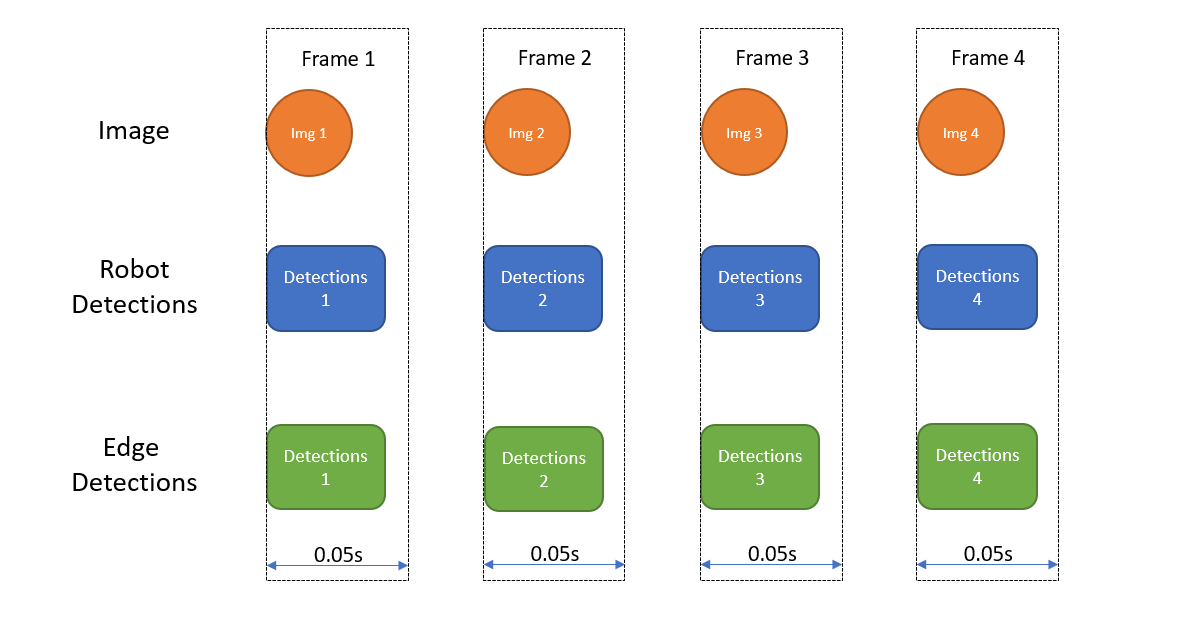
\includegraphics[width=120mm]{figures/setup/sync_eval.png}
    \caption{Synchronous evaluation paradigm}
    \label{fig:sync_eval}
\end{figure}

\subsection{Asynchronous Evaluation Paradigm}

\begin{figure}[htp]
    \centering
    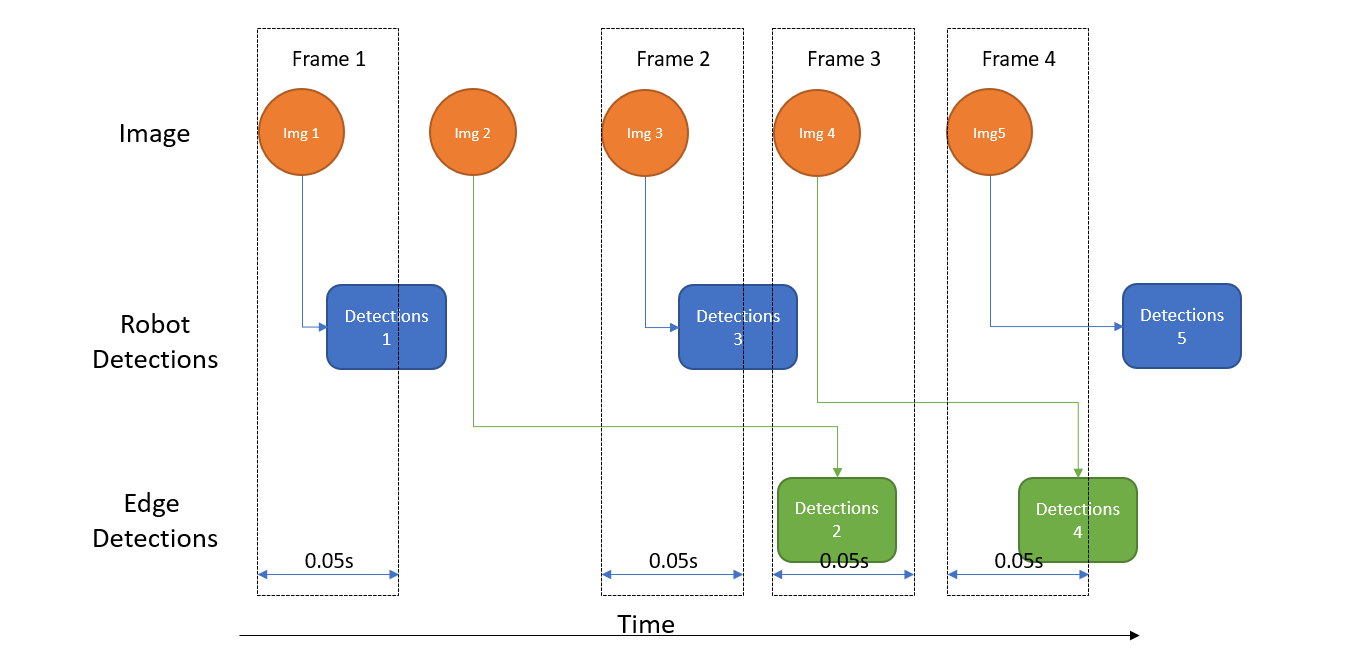
\includegraphics[width=120mm]{figures/setup/async_eval.png}
    \caption{Asynchronous evaluation paradigm}
    \label{fig:async_eval}
\end{figure}

\subsection{Discussion on Evaluation Methods}
\chapter{Simulation}\label{ch:simulation}

\section{Results and Discussion}
\chapter{Real-Robot Experiment}

\section{Experiment Setup}

\section{Results and Discussion}

\chapter{Conclusion and Future Works}\label{ch:conclusion_and_future_works}
\chapter{Acknowledgement}

%
% Appendix
% --------
\appendix%
\chapter{Appendix 1}%
\Blindtext%
%
%
%
%
% References
% ----------
{%
    %\sloppy% "Word"-like typesetting in order to improve breaking lines with long URLs/DOIs
    \printbibliography[heading=bibintoc]%
}%
%
%
\end{document}%
%
%
